% Created by tikzDevice version 0.12.6 on 2026-05-14 10:51:13
% !TEX encoding = UTF-8 Unicode
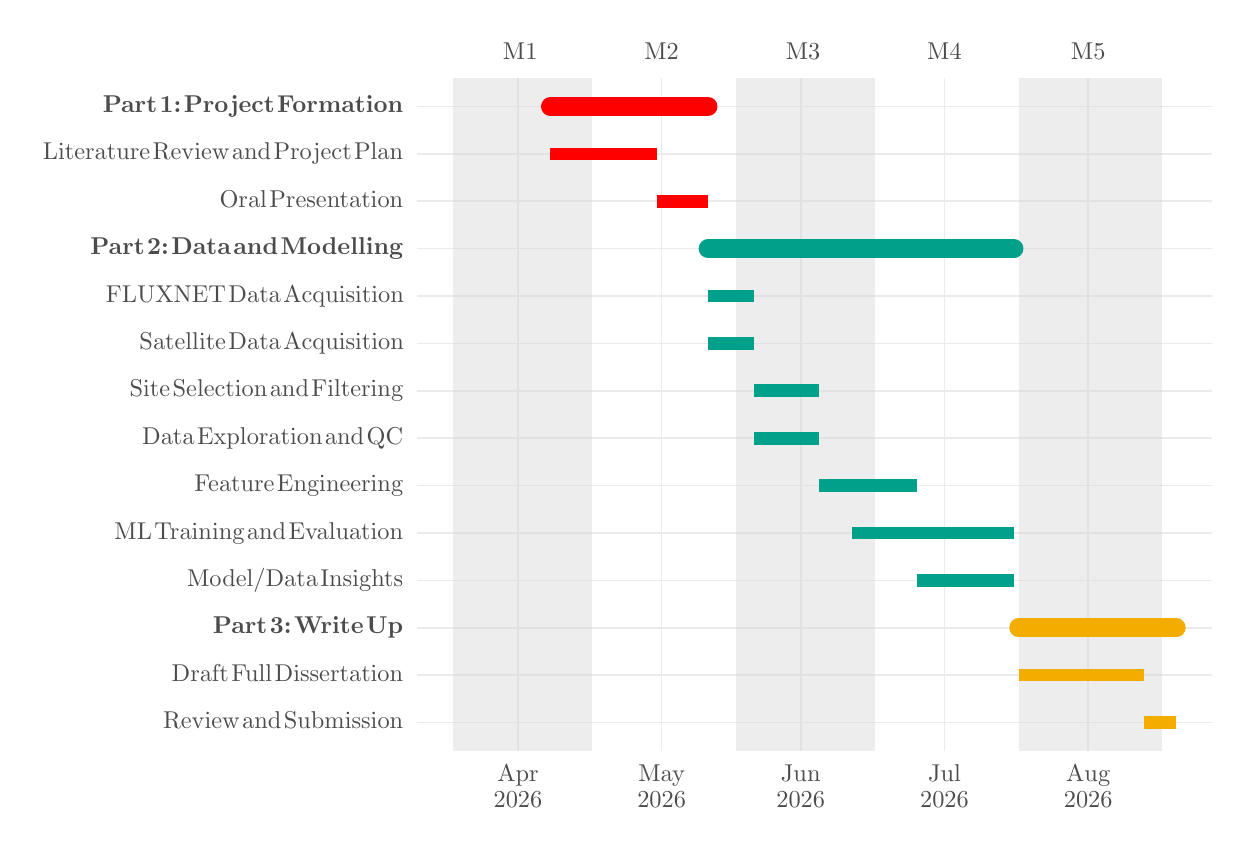
\begin{tikzpicture}[x=1pt,y=1pt]
\definecolor{fillColor}{RGB}{255,255,255}
\path[use as bounding box,fill=fillColor,fill opacity=0.00] (0,0) rectangle (433.62,289.08);
\begin{scope}
\path[clip] (  0.00,  0.00) rectangle (433.62,289.08);
\definecolor{fillColor}{RGB}{255,255,255}

\path[fill=fillColor] (  0.00,  0.00) rectangle (433.62,289.08);
\end{scope}
\begin{scope}
\path[clip] (140.64, 27.73) rectangle (428.12,270.86);
\definecolor{drawColor}{gray}{0.92}

\path[draw=drawColor,line width= 0.6pt,line join=round] (140.64, 38.00) --
	(428.12, 38.00);

\path[draw=drawColor,line width= 0.6pt,line join=round] (140.64, 55.12) --
	(428.12, 55.12);

\path[draw=drawColor,line width= 0.6pt,line join=round] (140.64, 72.24) --
	(428.12, 72.24);

\path[draw=drawColor,line width= 0.6pt,line join=round] (140.64, 89.36) --
	(428.12, 89.36);

\path[draw=drawColor,line width= 0.6pt,line join=round] (140.64,106.49) --
	(428.12,106.49);

\path[draw=drawColor,line width= 0.6pt,line join=round] (140.64,123.61) --
	(428.12,123.61);

\path[draw=drawColor,line width= 0.6pt,line join=round] (140.64,140.73) --
	(428.12,140.73);

\path[draw=drawColor,line width= 0.6pt,line join=round] (140.64,157.85) --
	(428.12,157.85);

\path[draw=drawColor,line width= 0.6pt,line join=round] (140.64,174.98) --
	(428.12,174.98);

\path[draw=drawColor,line width= 0.6pt,line join=round] (140.64,192.10) --
	(428.12,192.10);

\path[draw=drawColor,line width= 0.6pt,line join=round] (140.64,209.22) --
	(428.12,209.22);

\path[draw=drawColor,line width= 0.6pt,line join=round] (140.64,226.34) --
	(428.12,226.34);

\path[draw=drawColor,line width= 0.6pt,line join=round] (140.64,243.46) --
	(428.12,243.46);

\path[draw=drawColor,line width= 0.6pt,line join=round] (140.64,260.59) --
	(428.12,260.59);

\path[draw=drawColor,line width= 0.6pt,line join=round] (177.16, 27.73) --
	(177.16,270.86);

\path[draw=drawColor,line width= 0.6pt,line join=round] (229.09, 27.73) --
	(229.09,270.86);

\path[draw=drawColor,line width= 0.6pt,line join=round] (279.35, 27.73) --
	(279.35,270.86);

\path[draw=drawColor,line width= 0.6pt,line join=round] (331.29, 27.73) --
	(331.29,270.86);

\path[draw=drawColor,line width= 0.6pt,line join=round] (383.22, 27.73) --
	(383.22,270.86);
\definecolor{fillColor}{RGB}{211,211,211}

\path[fill=fillColor,fill opacity=0.40] (153.70, 27.73) rectangle (203.96,270.86);

\path[fill=fillColor,fill opacity=0.40] (255.90, 27.73) rectangle (306.16,270.86);

\path[fill=fillColor,fill opacity=0.40] (358.09, 27.73) rectangle (410.03,270.86);
\definecolor{drawColor}{RGB}{242,173,0}

\path[draw=drawColor,line width= 4.6pt,line join=round] (403.33, 38.00) -- (415.05, 38.00);

\path[draw=drawColor,line width= 4.6pt,line join=round] (358.09, 55.12) -- (403.33, 55.12);

\path[] (358.09, 72.24) -- (415.05, 72.24);
\definecolor{drawColor}{RGB}{0,160,138}

\path[draw=drawColor,line width= 4.6pt,line join=round] (321.23, 89.36) -- (356.42, 89.36);

\path[draw=drawColor,line width= 4.6pt,line join=round] (297.78,106.49) -- (356.42,106.49);

\path[draw=drawColor,line width= 4.6pt,line join=round] (286.05,123.61) -- (321.23,123.61);

\path[draw=drawColor,line width= 4.6pt,line join=round] (262.60,140.73) -- (286.05,140.73);

\path[draw=drawColor,line width= 4.6pt,line join=round] (262.60,157.85) -- (286.05,157.85);

\path[draw=drawColor,line width= 4.6pt,line join=round] (245.85,174.98) -- (262.60,174.98);

\path[draw=drawColor,line width= 4.6pt,line join=round] (245.85,192.10) -- (262.60,192.10);

\path[] (245.85,209.22) -- (356.42,209.22);
\definecolor{drawColor}{RGB}{255,0,0}

\path[draw=drawColor,line width= 4.6pt,line join=round] (227.42,226.34) -- (245.85,226.34);

\path[draw=drawColor,line width= 4.6pt,line join=round] (188.88,243.46) -- (227.42,243.46);

\path[] (188.88,260.59) -- (245.85,260.59);

\path[] (403.33, 38.00) -- (415.05, 38.00);

\path[] (358.09, 55.12) -- (403.33, 55.12);
\definecolor{drawColor}{RGB}{242,173,0}

\path[draw=drawColor,line width= 6.8pt,line join=round,line cap=round] (358.09, 72.24) -- (415.05, 72.24);

\path[] (321.23, 89.36) -- (356.42, 89.36);

\path[] (297.78,106.49) -- (356.42,106.49);

\path[] (286.05,123.61) -- (321.23,123.61);

\path[] (262.60,140.73) -- (286.05,140.73);

\path[] (262.60,157.85) -- (286.05,157.85);

\path[] (245.85,174.98) -- (262.60,174.98);

\path[] (245.85,192.10) -- (262.60,192.10);
\definecolor{drawColor}{RGB}{0,160,138}

\path[draw=drawColor,line width= 6.8pt,line join=round,line cap=round] (245.85,209.22) -- (356.42,209.22);

\path[] (227.42,226.34) -- (245.85,226.34);

\path[] (188.88,243.46) -- (227.42,243.46);
\definecolor{drawColor}{RGB}{255,0,0}

\path[draw=drawColor,line width= 6.8pt,line join=round,line cap=round] (188.88,260.59) -- (245.85,260.59);
\end{scope}
\begin{scope}
\path[clip] (  0.00,  0.00) rectangle (433.62,289.08);
\definecolor{drawColor}{gray}{0.30}

\node[text=drawColor,anchor=base,inner sep=0pt, outer sep=0pt, scale=  0.88] at (177.99,277.52) {M1};

\node[text=drawColor,anchor=base,inner sep=0pt, outer sep=0pt, scale=  0.88] at (229.09,277.52) {M2};

\node[text=drawColor,anchor=base,inner sep=0pt, outer sep=0pt, scale=  0.88] at (280.19,277.52) {M3};

\node[text=drawColor,anchor=base,inner sep=0pt, outer sep=0pt, scale=  0.88] at (331.29,277.52) {M4};

\node[text=drawColor,anchor=base,inner sep=0pt, outer sep=0pt, scale=  0.88] at (383.22,277.52) {M5};
\end{scope}
\begin{scope}
\path[clip] (  0.00,  0.00) rectangle (433.62,289.08);
\definecolor{drawColor}{gray}{0.30}

\node[text=drawColor,anchor=base west,inner sep=0pt, outer sep=0pt, scale=  0.88] at ( 48.90, 35.82) {Review};

\node[text=drawColor,anchor=base west,inner sep=0pt, outer sep=0pt, scale=  0.88] at ( 77.52, 35.82) {and};

\node[text=drawColor,anchor=base west,inner sep=0pt, outer sep=0pt, scale=  0.88] at ( 92.58, 35.82) {Submission};
\end{scope}
\begin{scope}
\path[clip] (  0.00,  0.00) rectangle (433.62,289.08);
\definecolor{drawColor}{gray}{0.30}

\node[text=drawColor,anchor=base west,inner sep=0pt, outer sep=0pt, scale=  0.88] at ( 52.03, 52.95) {Draft};

\node[text=drawColor,anchor=base west,inner sep=0pt, outer sep=0pt, scale=  0.88] at ( 73.59, 52.95) {Full};

\node[text=drawColor,anchor=base west,inner sep=0pt, outer sep=0pt, scale=  0.88] at ( 89.25, 52.95) {Dissertation};
\end{scope}
\begin{scope}
\path[clip] (  0.00,  0.00) rectangle (433.62,289.08);
\definecolor{drawColor}{gray}{0.30}

\node[text=drawColor,anchor=base west,inner sep=0pt, outer sep=0pt, scale=  0.88] at ( 66.95, 70.06) {\bfseries Part};

\node[text=drawColor,anchor=base west,inner sep=0pt, outer sep=0pt, scale=  0.88] at ( 87.49, 70.06) {\bfseries 3:};

\node[text=drawColor,anchor=base west,inner sep=0pt, outer sep=0pt, scale=  0.88] at ( 96.24, 70.06) {\bfseries Write};

\node[text=drawColor,anchor=base west,inner sep=0pt, outer sep=0pt, scale=  0.88] at (122.28, 70.06) {\bfseries Up};
\end{scope}
\begin{scope}
\path[clip] (  0.00,  0.00) rectangle (433.62,289.08);
\definecolor{drawColor}{gray}{0.30}

\node[text=drawColor,anchor=base west,inner sep=0pt, outer sep=0pt, scale=  0.88] at ( 57.60, 87.19) {Model/Data};

\node[text=drawColor,anchor=base west,inner sep=0pt, outer sep=0pt, scale=  0.88] at (105.77, 87.19) {Insights};
\end{scope}
\begin{scope}
\path[clip] (  0.00,  0.00) rectangle (433.62,289.08);
\definecolor{drawColor}{gray}{0.30}

\node[text=drawColor,anchor=base west,inner sep=0pt, outer sep=0pt, scale=  0.88] at ( 31.36,104.31) {ML};

\node[text=drawColor,anchor=base west,inner sep=0pt, outer sep=0pt, scale=  0.88] at ( 45.80,104.31) {Training};

\node[text=drawColor,anchor=base west,inner sep=0pt, outer sep=0pt, scale=  0.88] at ( 79.21,104.31) {and};

\node[text=drawColor,anchor=base west,inner sep=0pt, outer sep=0pt, scale=  0.88] at ( 94.26,104.31) {Evaluation};
\end{scope}
\begin{scope}
\path[clip] (  0.00,  0.00) rectangle (433.62,289.08);
\definecolor{drawColor}{gray}{0.30}

\node[text=drawColor,anchor=base west,inner sep=0pt, outer sep=0pt, scale=  0.88] at ( 60.22,121.43) {Feature};

\node[text=drawColor,anchor=base west,inner sep=0pt, outer sep=0pt, scale=  0.88] at ( 90.08,121.43) {Engineering};
\end{scope}
\begin{scope}
\path[clip] (  0.00,  0.00) rectangle (433.62,289.08);
\definecolor{drawColor}{gray}{0.30}

\node[text=drawColor,anchor=base west,inner sep=0pt, outer sep=0pt, scale=  0.88] at ( 41.38,138.56) {Data};

\node[text=drawColor,anchor=base west,inner sep=0pt, outer sep=0pt, scale=  0.88] at ( 61.20,138.56) {Exploration};

\node[text=drawColor,anchor=base west,inner sep=0pt, outer sep=0pt, scale=  0.88] at (107.43,138.56) {and};

\node[text=drawColor,anchor=base west,inner sep=0pt, outer sep=0pt, scale=  0.88] at (122.49,138.56) {QC};
\end{scope}
\begin{scope}
\path[clip] (  0.00,  0.00) rectangle (433.62,289.08);
\definecolor{drawColor}{gray}{0.30}

\node[text=drawColor,anchor=base west,inner sep=0pt, outer sep=0pt, scale=  0.88] at ( 36.85,155.68) {Site};

\node[text=drawColor,anchor=base west,inner sep=0pt, outer sep=0pt, scale=  0.88] at ( 52.40,155.68) {Selection};

\node[text=drawColor,anchor=base west,inner sep=0pt, outer sep=0pt, scale=  0.88] at ( 87.49,155.68) {and};

\node[text=drawColor,anchor=base west,inner sep=0pt, outer sep=0pt, scale=  0.88] at (102.55,155.68) {Filtering};
\end{scope}
\begin{scope}
\path[clip] (  0.00,  0.00) rectangle (433.62,289.08);
\definecolor{drawColor}{gray}{0.30}

\node[text=drawColor,anchor=base west,inner sep=0pt, outer sep=0pt, scale=  0.88] at ( 40.40,172.80) {Satellite};

\node[text=drawColor,anchor=base west,inner sep=0pt, outer sep=0pt, scale=  0.88] at ( 72.56,172.80) {Data};

\node[text=drawColor,anchor=base west,inner sep=0pt, outer sep=0pt, scale=  0.88] at ( 92.38,172.80) {Acquisition};
\end{scope}
\begin{scope}
\path[clip] (  0.00,  0.00) rectangle (433.62,289.08);
\definecolor{drawColor}{gray}{0.30}

\node[text=drawColor,anchor=base west,inner sep=0pt, outer sep=0pt, scale=  0.88] at ( 28.30,189.92) {FLUXNET};

\node[text=drawColor,anchor=base west,inner sep=0pt, outer sep=0pt, scale=  0.88] at ( 72.56,189.92) {Data};

\node[text=drawColor,anchor=base west,inner sep=0pt, outer sep=0pt, scale=  0.88] at ( 92.38,189.92) {Acquisition};
\end{scope}
\begin{scope}
\path[clip] (  0.00,  0.00) rectangle (433.62,289.08);
\definecolor{drawColor}{gray}{0.30}

\node[text=drawColor,anchor=base west,inner sep=0pt, outer sep=0pt, scale=  0.88] at ( 22.64,207.04) {\bfseries Part};

\node[text=drawColor,anchor=base west,inner sep=0pt, outer sep=0pt, scale=  0.88] at ( 43.17,207.04) {\bfseries 2:};

\node[text=drawColor,anchor=base west,inner sep=0pt, outer sep=0pt, scale=  0.88] at ( 51.92,207.04) {\bfseries Data};

\node[text=drawColor,anchor=base west,inner sep=0pt, outer sep=0pt, scale=  0.88] at ( 74.33,207.04) {\bfseries and};

\node[text=drawColor,anchor=base west,inner sep=0pt, outer sep=0pt, scale=  0.88] at ( 91.37,207.04) {\bfseries Modelling};
\end{scope}
\begin{scope}
\path[clip] (  0.00,  0.00) rectangle (433.62,289.08);
\definecolor{drawColor}{gray}{0.30}

\node[text=drawColor,anchor=base west,inner sep=0pt, outer sep=0pt, scale=  0.88] at ( 69.33,224.17) {Oral};

\node[text=drawColor,anchor=base west,inner sep=0pt, outer sep=0pt, scale=  0.88] at ( 87.35,224.17) {Presentation};
\end{scope}
\begin{scope}
\path[clip] (  0.00,  0.00) rectangle (433.62,289.08);
\definecolor{drawColor}{gray}{0.30}

\node[text=drawColor,anchor=base west,inner sep=0pt, outer sep=0pt, scale=  0.88] at (  5.50,241.29) {Literature};

\node[text=drawColor,anchor=base west,inner sep=0pt, outer sep=0pt, scale=  0.88] at ( 45.16,241.29) {Review};

\node[text=drawColor,anchor=base west,inner sep=0pt, outer sep=0pt, scale=  0.88] at ( 73.78,241.29) {and};

\node[text=drawColor,anchor=base west,inner sep=0pt, outer sep=0pt, scale=  0.88] at ( 88.84,241.29) {Project};

\node[text=drawColor,anchor=base west,inner sep=0pt, outer sep=0pt, scale=  0.88] at (117.97,241.29) {Plan};
\end{scope}
\begin{scope}
\path[clip] (  0.00,  0.00) rectangle (433.62,289.08);
\definecolor{drawColor}{gray}{0.30}

\node[text=drawColor,anchor=base west,inner sep=0pt, outer sep=0pt, scale=  0.88] at ( 27.13,258.40) {\bfseries Part};

\node[text=drawColor,anchor=base west,inner sep=0pt, outer sep=0pt, scale=  0.88] at ( 47.67,258.40) {\bfseries 1:};

\node[text=drawColor,anchor=base west,inner sep=0pt, outer sep=0pt, scale=  0.88] at ( 56.42,258.40) {\bfseries Project};

\node[text=drawColor,anchor=base west,inner sep=0pt, outer sep=0pt, scale=  0.88] at ( 90.16,258.40) {\bfseries Formation};
\end{scope}
\begin{scope}
\path[clip] (  0.00,  0.00) rectangle (433.62,289.08);
\definecolor{drawColor}{gray}{0.30}

\node[text=drawColor,anchor=base,inner sep=0pt, outer sep=0pt, scale=  0.88] at (177.16, 16.71) {Apr};

\node[text=drawColor,anchor=base,inner sep=0pt, outer sep=0pt, scale=  0.88] at (177.16,  7.21) {2026};

\node[text=drawColor,anchor=base,inner sep=0pt, outer sep=0pt, scale=  0.88] at (229.09, 16.71) {May};

\node[text=drawColor,anchor=base,inner sep=0pt, outer sep=0pt, scale=  0.88] at (229.09,  7.21) {2026};

\node[text=drawColor,anchor=base,inner sep=0pt, outer sep=0pt, scale=  0.88] at (279.35, 16.71) {Jun};

\node[text=drawColor,anchor=base,inner sep=0pt, outer sep=0pt, scale=  0.88] at (279.35,  7.21) {2026};

\node[text=drawColor,anchor=base,inner sep=0pt, outer sep=0pt, scale=  0.88] at (331.29, 16.71) {Jul};

\node[text=drawColor,anchor=base,inner sep=0pt, outer sep=0pt, scale=  0.88] at (331.29,  7.21) {2026};

\node[text=drawColor,anchor=base,inner sep=0pt, outer sep=0pt, scale=  0.88] at (383.22, 16.71) {Aug};

\node[text=drawColor,anchor=base,inner sep=0pt, outer sep=0pt, scale=  0.88] at (383.22,  7.21) {2026};
\end{scope}
\end{tikzpicture}
